\section{Grundbegriffe}
	
		\subsection{DC- und Kleinsignal-Ersatzschaltung}
			\begin{tabular}{|p{4.3cm}|p{3.93cm}|p{4.5cm}|p{4.5cm}|}
			\hline
			& \footnotesize{\textbf{DC-Ersatzschaltung}} 
			& \footnotesize{\textbf{Kleinsignal-Ersatztschaltung mit L und C}}	
			& \footnotesize{\textbf{Kleinsignal-Ersatztschaltung ohne L\footnotemark[1] und C\footnotemark[2]}}
			\\ \hline
			\footnotesize{\textbf{Gleichspannungsquelle (V)}} 
			& \cellcolor{lightgrey}Übernehmen 
			& Kurzschliessen\footnotemark[3] 
			& Kurzschliessen\footnotemark[3] 
			\\ \hline
			\footnotesize{\textbf{Gleichstromquelle (I)}} 
			& \cellcolor{lightgrey}Übernehmen 
			& Entfernen\footnotemark[4] 
			& Entfernen\footnotemark[4] 
			\\ \hline
			\footnotesize{\textbf{Wechselspannungsquelle (v)}} 
			& Kurzschliessen\footnotemark[3] 
			& \cellcolor{lightgrey}Übernehmen 
			& \cellcolor{lightgrey}Übernehmen
			\\ \hline
			\footnotesize{\textbf{Wechselstromquelle (i)}} 
			& Entfernen\footnotemark[4] 
			& \cellcolor{lightgrey}Übernehmen 
			& \cellcolor{lightgrey}Übernehmen
			\\ \hline
			\footnotesize{\textbf{L}} 
			& Kurzschliessen\footnotemark[5] 
			& \cellcolor{lightgrey}Übernehmen 
			& Entfernen wenn L ``sehr gross''\footnotemark[1]
			\\ \hline
			\footnotesize{\textbf{C}} 
			& Entfernen\footnotemark[6] 
			& \cellcolor{lightgrey}Übernehmen 
			& Kurzschliessen wenn C ``sehr gross''\footnotemark[2]
			\\ \hline
			\footnotesize{\textbf{Nichtlineares Bauteil}} (im Beispiel die Diode $D_1$) 
			& Ersetzten durch die DC-Ersatztschaltung des nichtlinearen Bauteils
			& Ersetzten durch die Kleinsignal-Ersatzschaltung des nichtlinearen Bauteils
			& Ersetzten durch die Kleinsignal-Ersatzschaltung des nichtlinearen Bauteils
			\\ \hline
			\textbf{Beispiel:} Signalabschwächer mit Diode
			& Die DC-Ersatzschaltung der Diode ist eine Spannungsquelle von $V_D = 0.6V$
			& Die Kleinsignal-Ersatz"-schaltung der Diode ist ein Wiederstand $r_D$ (wobei $r_D = 26 \frac{mv}{I_D}$)
			& 
			\\
			\parbox[c][3cm]{4.25cm}{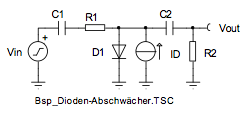
\includegraphics[width=4.25cm]{./bilder/dc-kleinsignal-ersatz-beispiel.png}}
			& \parbox[c][3cm]{3.8cm}{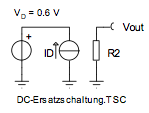
\includegraphics[width=3.8cm]{./bilder/dc-kleinsignal-ersatz-dc.png}}
			& \parbox[c][3cm]{4.5cm}{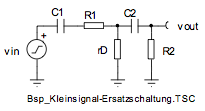
\includegraphics[width=4.5cm]{./bilder/dc-kleinsignal-ersatz-LC.png}}
			& \parbox[c][3cm]{4.5cm}{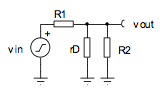
\includegraphics[width=4.5cm]{./bilder/dc-kleinsignal-ersatz-ohneLC.png}}
			\\ \hline
			\end{tabular}
			%}
			\footnotetext[1]{L ist eine Sperrdrossel}
			\footnotetext[2]{C ist ein Koppel- oder Bypass-Kondensator}
			\footnotetext[3]{weil $r_{Quelle} = 0\Omega$}
			\footnotetext[4]{weil $r_{Quelle} = \infty\Omega$}
			\footnotetext[5]{weil $r_{DC} = 0\Omega$}
			\footnotetext[6]{weil $r_{AC} = \infty\Omega$}
			

		\subsection{Verstärkertypen}
			\begin{minipage}{10cm}
            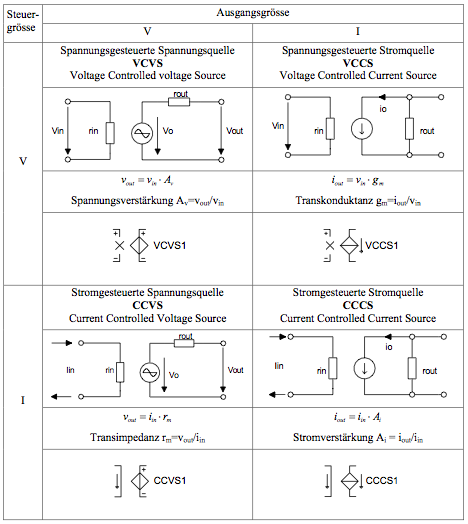
\includegraphics[width=10cm]{./bilder/verstaerkertypen.png}
            \end{minipage}
			\begin{minipage}{8cm}
            {\bf Verstärkerfaktoren:}\\
            - Spannungs-Verstärkerfaktor \hspace{4mm}$A_v$ (ohne Einheit)\\
            - Strom-Verstärkungsfaktor \hspace{6mm} $A_i$ (ohne Einheit)\\
            - Transkonduktanz \hspace{19mm} $g_m$ (Einheit $\Omega^{-1}$)\\
            - Transresistanz \hspace{24mm} $r_m$ (Einheit $\Omega$)\\ \\
            Dynam. Eingangswiderstand \hspace{5mm} $r_{in}$ ($\Omega$)\\
            Dynam. Ausgangswiderstand \hspace{4mm} $r_{out}$ ($\Omega$)\\ \\
            {\bf Bei idealen gesteuerten Quellen gelten folgende Werte für
            $r_{in}$ und $r_{out}$:}\\
            Bei Stromsteuerung ist \hspace{13.5mm} $r_{in}=0 \Omega$\\
            Bei Spannungssteuerung ist \hspace{6.5mm} $r_{in}=\infty \Omega$\\
            Beim Stromausgang ist \hspace{13.5mm} $r_{out}=\infty \Omega$\\
            Beim Spannungsausgang ist \hspace{6.5mm} $r_{out}=0 \Omega$\\
            
            {\bf Invertierender Verstärker:}\\
            Verstarkungsfaktor ist negativ $(A<0)$\\
            $v_{out}$ verläuft {\it gegenphasig} zu $v_{in}$\\
            
            {\bf Nichtinvertierender Verstärker:}\\
            Verstärkungsfaktor ist positiv $(A>0)$\\
            $v_{out}$ verläuft {\it gleichphasig} zu $v_{in}$
            \end{minipage}
	
	
		\subsection{Dezibel (dB)}
			\begin{tabular}{p{10cm}p{8cm}}
        		Das Dezibel der Verhältniszahl $V$ wird wie folgt berechnet:
        		& \fbox{$V_{dB}=20 log \left| V\right|$}\\
        		Aus der gegebenen Dezibel-Zahl $V_{dB}\to$ lineare Verhältniszahl:
        		& \fbox{$V=10^{\frac{V_{dB}}{20dB}}$}\\ \\
        \end{tabular}

		\subsection{Übertragungsfaktoren}
			\begin{minipage}{18cm}
	   	    	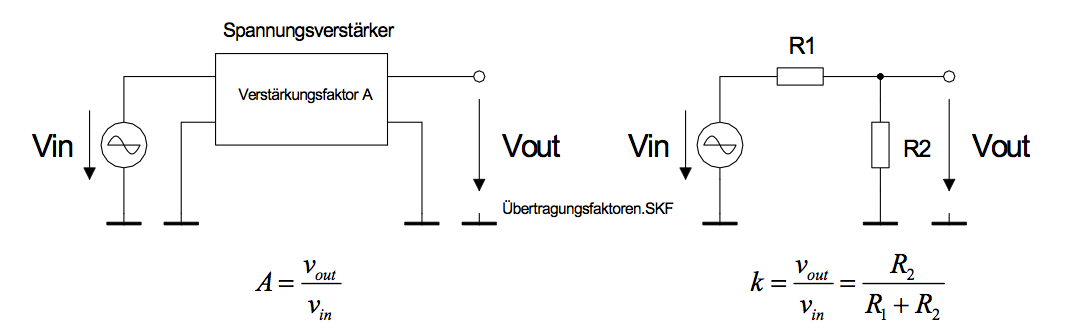
\includegraphics[width=16cm]{./bilder/uebertragungsfaktoren.png}
       		\end{minipage}

		\subsection{Grosssignalwiderstand}
			Gleichstromwiderstand $R$ \hspace{15mm} $R=\frac{V_R}{I_R}$
			$\left(\frac{\mbox{Gleichspannung im Arbeitspunkt}}{\mbox{Gleichstrom im
			Arbeitspunkt}}\right)$\\ \\
			Bei {\it linearen Widerständen} hängt der Grosssignalwiderstand
			{\it nicht} vom Arbeitspunkt ab.\\
			Bei {\it nicht linearen Widerständen} hängt der Grosssignalwiderstand
			vom Arbeitspunkt ab. $\Rightarrow$ Interessiert aber in der Elektronik nicht.
			Sind immer am Kleinsignalwiderstand $r$ intressiert.\\

		\subsection{Kleinsignalwiderstand (dynamischer oder differenzieller
		Widerstand)}
			Kleinsignalwiderstand $r$ \hspace{15mm} $r_L=\frac{dV_L}{dI_L}$ In der Praxis
			verwenden wir die Näherung $r_L=\frac{dV_L}{dI_L}\approx \frac{\Delta
			V_L}{\Delta I_L}$\\ \\
			Wenn die Strom-Spannungskennlinie $V=f(I)$ mathematisch gegeben ist, erhalten
			wir den Kleinsignalwiderstand $r_L$ durch Differenzierung der
			Kennliniengleichung $V_L=f(I_L)$ im Arbeitspunkt $(I_L, V_L)$.\\
			Bei {\it nichtlinearen Zweipolen} hängt der Kleinsignalwiderstand $r$
			vom Arbeitspunkt ab, aber $r\neq R$\\
			Bei {\it linearen Zweipolen} ist der Kleinsignalwiderstand $r$
			identisch mit dem DC-Widerstand $R$. Desshalb ist $r$ bei {\it linearen
			Zweipolen} vom Arbeitspunkt {\it unabhängig}.\\
		
	\subsection{Überlagerungssatz für lineare Systeme}
			Wenn das Eingangssignal eines linearen Verstärkers (oder allgemein eines
			linearen Netzwerkes) aus einer Summe von zwei verschiedenen Signalen besteht,
			dürfen wir die beiden Teilsignale getrennt mit dem Verstärkungsfaktor
			multiplizieren und die beiden resultierenden Ausgangssignale am Ausgang
			addieren.\\
			\hspace*{10mm}
			\fbox{$v_{out \hspace{1mm}
			total}=(v_{in1}+v_{in2})A=v_{in1}A+v_{in2}A=v_{out1}+v_{out2}=v_{in
			\hspace{1mm}total}A$}\\